\chapter{Project Management}\label{ch:schedule}

    \section{Team Roles} Within this section we will detail roles needed to be fulfilled within our team that aligns
    with the context of our project and our chosen software lifecycle methodology.\ Each role will be assigned team
    members that are responsible for the tasks being undertaken by said role.\ Due to the nature of our scrum methodology,
    we will be avoiding the use of a designated team leader and instead opting for a self-managing team~\cite{parafianowicz_2019}.
     A list of our team roles can be seen below, along with their assignees and detail about
    what each role entails.

        \subsection{Scrum Master} \textbf{Assignee: } Sean Coaker\newline \textbf{Description: } The scrum master within
        our project will not act as a team leader, but will instead facilitate and manage the process of the scrum
        software lifecycle methodology \cite{bass_2014}.\ Due to the adjustments we made to our scrum methodology, such
        as avoiding daily meetings due to university commitments, our scrum master will need to ensure that our team
        adheres to our adjusted methodology and time plan set out within this document.\ Therefore, our scrum master will
        need a clear understanding of the team's selected software lifecycle methodology and should regularly reference
        it to provide consistent guidance to the team when developing the project.

        \subsection{Full Stack Developer} \textbf{Assignee: } All Team Members (Sean Coaker, Pedro Caetano, Matthew
        Culley, Panayiotis Melios)\newline \textbf{Description: } Our full stack developers will handle the code
        development for all aspects of the project.\ They will develop code for both the walking aid and wearable
        devices, implementing code that allows our project to meet the functional and non-functional requirements
        detailed within this document. The developers will need to quickly adjust to the new software and hardware they
        encounter during the development of this project to ensure that the final product is developed on time. As
        mentioned previously, our team is self-managed and therefore regular communication will need to occur between
        developers to keep everyone up to date with progress being made.

        \subsection{Communications Officer} \textbf{Assignee: } Sean Coaker\newline \textbf{Description: } To provide
        communication between the development team and the client, we elected a communications officer. The
        communcations officer shall be the main point of contact with the client, dealing with queries, organising
        meetings and ensuring that the client requirements are communicated correctly to the development team. The
        communcations officer has so far organised initial meetings with the client, and submitted documented user
        requirements to the client, which the client confirmed they are content with.

        \subsection{Prototype Design Officer} \textbf{Assignee: } Pedro Caetano\newline \textbf{Description: } Due to
        the nature of our project, we needed to assign a prototype design officer to handle the design and development
        process of the device casing. We elected Pedro for this due to his previous experience in working with 3D
        printers and feel that his experience can transfer well into developing the designs for our device casing, along
        with being able to transfer these designs into 3D printed useable prototypes.

        \subsection{Testers including Quality Assurance responsibilities} \textbf{Assignee: } All Team Members (Sean Coaker, Pedro Caetano, Matthew Culley, Panayiotis Melios)\newline \textbf{Description: } As mentioned previously, our team is self-managed meaning we wanted to avoid the use of leadership roles such as team leaders, testing leaders and quality assurance leaders. For this role, all team members will be expected to perform testing procedures that align with our testing strategy. Along with this, each team member will also take on quality assurance responsibilities to ensure that our product is of the highest quality the team can produce. Our testing role also includes the responsibilities of documenting test results to allow the team to collate them at the development of our milestone 3 document for proof of the success of our product.

        \subsection{Documentation Developers} \textbf{Assignee: } All Team Members (Sean Coaker, Pedro Caetano, Matthew Culley, Panayiotis Melios)\newline \textbf{Description: } As we are a small team, it is a requirement that all team members contribute to the development of the documentation required to be completed within this project. The fact that all members assigned to the development of the documentation are also full-stack developers can be beneficial here as they can provide an in-depth understanding of the developed system when detailing it within our documentation.

    \section{Time Plan}

        \subsection{Gantt Chart} We built a Gantt Chart for the project schedule to allow us to keep track of the time.
        We couldn't create tasks that would indicate a slippage since it would disrupt the critical path. As a result,
        we increased the time alloted to each assignment, reflecting the slippage. We included slippage due of other
        university homework, exams and even illness.

            As shown in Figure \ref{fig:gantt_chart}, the highlighted tasks illustrate the project's critical path. We
            devided the project into three Sprints because we are utilizing the scrum methodlogy. The first Sprint
            consists only of require collection and project planning. The second Sprint includes the sprint plan, as
            well as the software and hadrware designs and implementations. The third Sprint contains the sprint plan as
            well as the system's final implementation, in which the walking aid will connect with our system, the wrist
            device. The final task of each Sprint is a milestone, signaling the Sprint's completion.

            \begin{figure}[H] 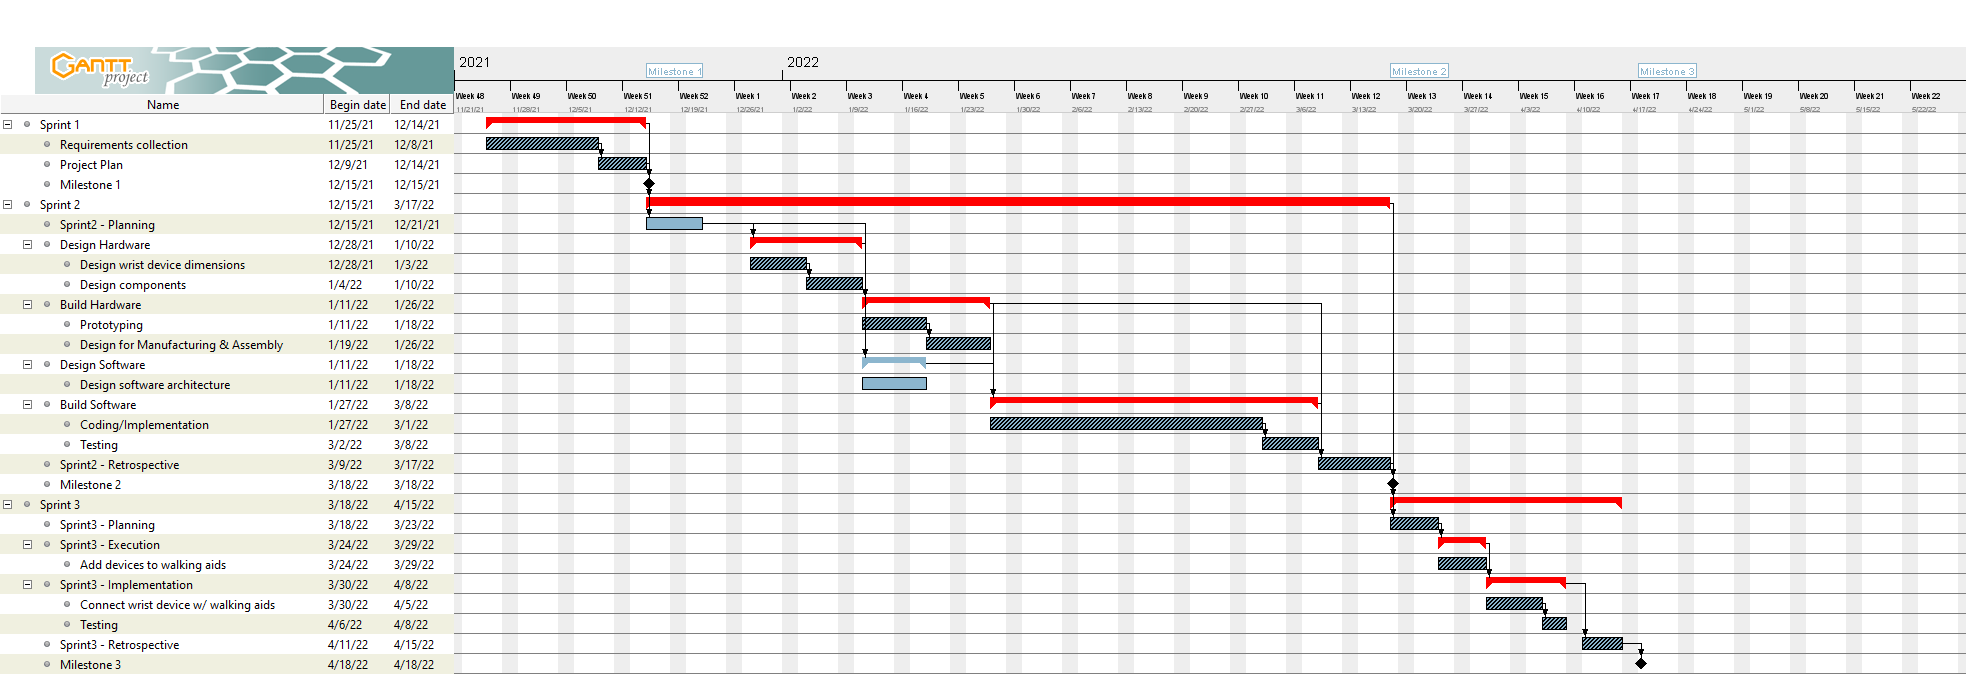
\includegraphics[width=\linewidth]{graphics/Gantt_Chart.png} \caption{Gantt Chart}
            \label{fig:gantt_chart} \end{figure}

        \subsection{Activity Network Diagram}

            In terms of scheduling, an activity diagram is just a significant as designing a Gantt Chart. We merged
            several of the jobs that were introduced to Gantt Chart into one task to make the activity network diagram
            more undestandable. However, this has no bearing on the total time requried to finish the project. According
            to Figure \ref{fig:activity_network_diagram}, the total time requried is 107 working days.

            \begin{figure}[H] 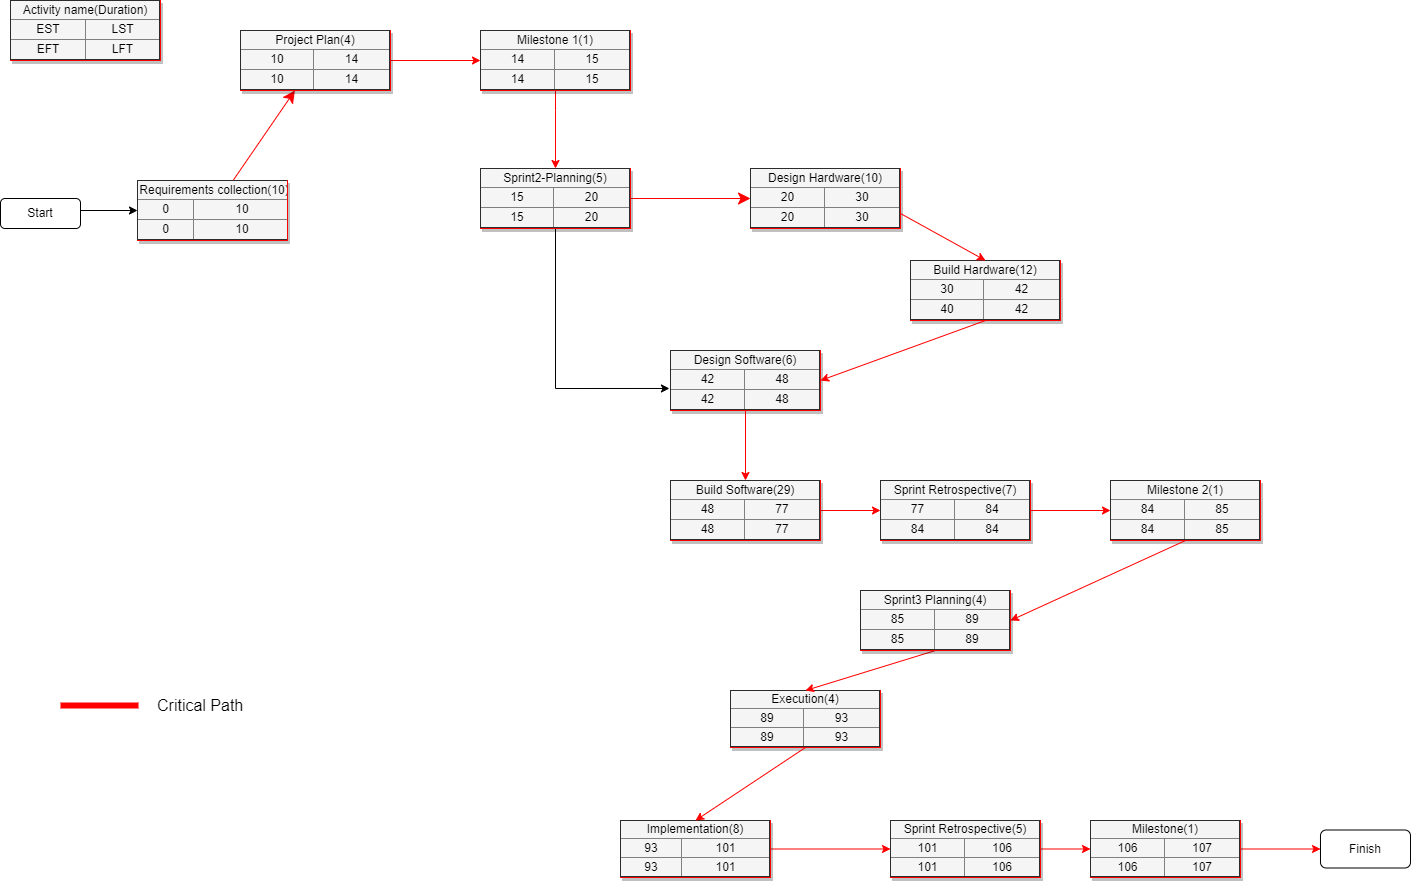
\includegraphics[width=\linewidth]{graphics/AND.drawio.png} \caption{Activity Network
            Diagram} \label{fig:activity_network_diagram} \end{figure}
